\documentclass[
pdftex,                %PDFtext verwenden
a4paper,                 %A4Papier
11pt,                     %Schriftgröße 12
parskip=half,         %Halbe Zeile Abstand zwischen den Paragraphen
headsepline,        %Linie nach Kopfzeile
]
{scrartcl}

\usepackage{graphicx}	% Paket um Grafiken einbetten zu können
\usepackage{color}	% Package für Farben im PDF
\usepackage{amsmath}
\usepackage{makeidx}	% Paket für die Indexerstellung
\usepackage[a4paper,left=2.0cm,right=2.0cm]{geometry}	%Paket zum Einstellen der Seitenränder
\usepackage[T1]{fontenc}	% Verwenden von T1 Fonts
\usepackage[urlcolor=blue]{hyperref}
\usepackage{caption}	% Caption verändern
\usepackage{verbatim}
\usepackage{booktabs}

%\setcapwidth[r]{\linewidth}

\begin{document}
	
	\newcommand{\group}{Group C - The Plebs}
	
	\newcommand{\header}{Python Chess AI}

	\pagestyle{myheadings}
	\markright{\group \hfill \header}
	
	\thispagestyle{empty}
	\begin{titlepage}

    Course: Project AI - Symbolic artificial intelligence \\
    Professor: Dr.-Ing. Stefan Fricke \\
    Semester: SOSE23 \\
    Date: 2023/07/26 \\

    Group Members: Who the fuck cares? \\
    Repository: https://github.com/PraxTube/chess-ai/ \\
		
		\vspace{8mm}
		
		\begin{center}
			
			{\Large \normalfont \bfseries Project Report} \\
			
			\vspace{5mm}
			
			{\Huge \normalfont \bfseries \header} \\
			\vspace{7mm}
			
			{\Large \normalfont \bfseries \group} \\
			\vspace{5mm}
			
		\end{center}
		\vspace{2cm}
		
		\begin{abstract}
			
			This is a dummy abstract.

Hello there.

			
		\end{abstract}
		
	\end{titlepage}
	
	\pagenumbering{Roman}
	
	\tableofcontents
	
	\pagebreak
	
	\pagenumbering{arabic}\setcounter{page}{1}

  \section{Introduction}

  Creating a chess AI from scratch is quite a challenging undertaking.
Not only will you need to write a whole chess backend, you will also
need to implement the AI features. One of the major issues here
is to write a chess backend without any bugs and to test your
AI properly to make sure the features you add actually make it
play better.

Our group chose to use Python for the whole project given
that that is what we were most familiar with.
The obvious trade-off here is of course that it's easy
to prototype but painfully slow and very error prone.
I personally would have liked to try to use Rust,
though in hindsight we would have probably abandoned
the project if we had used Rust simply because
the chess engine alone was so much work.
On the other side I have acquired some Rust experience
now and if I were to write the chess engine
(or something of a similar level) I would probably
go with Rust.

Regardless of our programming language, for version control
we obviously used git and to share our code base we used github.
The overall workflow here was pretty smooth.


  \pagebreak

  \section{Development}

  Before diving into the details of the
development process, it is beneficial to first provide an overview of the final product we created. Please note that comprehensive documentation can be accessed by clicking on the respective milestone name.

\begin{description}
  \item[\href{https://github.com/PraxTube/chess-ai/tree/master/docs/milestones/1-dummy-AI}{Mst1 - Dummy AI:}] \hfill
    \begin{itemize}
      \item Chess Backend
      \item Dummy AI (minimax)
      \item Basic Evaluation (Material only)
    \end{itemize}
  \item[\href{https://github.com/PraxTube/chess-ai/tree/master/docs/milestones/2-basic-AI}{Mst2 - Basic AI:}] \hfill
    \begin{itemize}
      \item Improve Backend
      \item Alpha-Beta Tree Search
      \item Improved Evaluation (PeSTO)
      \item Better time management
    \end{itemize}
  \item[\href{https://github.com/PraxTube/chess-ai/tree/master/docs/milestones/3-advanced-AI}{Mst3 - Advanced AI:}] \hfill
    \begin{itemize}
      \item Restructured Chess Backend
      \item Speed up Evaluation (through numpy)
      \item Improve move ordering
      \item Include King of the Hill in evaluation
      \item Restructure internal debug info
    \end{itemize}
  \item[\href{https://github.com/PraxTube/chess-ai/tree/master/docs/milestones/4-optimized-AI}{Mst4 Optimized AI:}] \hfill
    \begin{itemize}
      \item Improve evaluation
      \item Use Monte Carlo Tree Search
      \item Implement PVS/negamax
      \item Add Nullsearch
    \end{itemize}
\end{description}

\subsection{Mst1 Dummy AI}

The primary focus of this milestone was the development of the chess backend. Initially, we utilized the Python package python-chess\footnote{https://pypi.org/project/python-chess/}, which served as a valuable reference for structuring our own backend. We first implemented the AI using python-chess, and when we transitioned to our own backend, we were able to retain the structure provided by python-chess. Our backend was largely influenced by another repository\footnote{https://github.com/Jabezng2/Star-Wars-Chess-AI-Game} and a YouTube video\footnote{https://www.youtube.com/watch?v=EnYui0e73Rs}, which both provided crucial insights. Additionally, the Chess Programming website\footnote{https://www.chessprogramming.org/Chess} was an invaluable resource, offering a deeper understanding of the structure and functionality of a chess backend.

We conducted benchmarks on both our backend and the python-chess backend, with the intention of comparing their performance. Contrary to our expectations, our backend demonstrated superior speed. The reason for this remains unclear, but it was a reassuring outcome that bolstered our confidence to proceed with the project.

As this milestone was primarily focused on the backend, the main challenges and lessons learned were inherently linked to it. One significant issue was that the backend development was essentially a single-person task. While it might have been possible to divide the work between the AI and the backend, having multiple group members working on a single backend could lead to complications. Consequently, this task was undertaken by a single team member, resulting in over 900 lines of code in this milestone.

In this initial iteration of the backend, we focused on implementing the most essential features, leaving out the following:

\begin{itemize}
  \item{King of the hill condition}
  \item{En passant}
  \item{Only queen promotion}
  \item{Fen loading only semi-working}
\end{itemize}

The initial code base for the backend was admittedly disorganized, characterized by inconsistent naming conventions, redundant code, complex nested conditional and loop statements, and methods that were challenging to debug. However, this was anticipated and subsequently addressed in later milestones. It's worth noting that this approach aligns with a common software development strategy that has proven effective in my experience:

The strategy involves initially developing the software to follow the "happy path"\footnote{https://en.wikipedia.org/wiki/Happy\_path} until it functions as intended. Any potential restructuring of the code is undertaken as and when it is identified. Once this is accomplished, additional checks and validations can be incorporated. This approach was highly effective across all our milestones, essentially embodying a "fail-fast"\footnote{https://en.wikipedia.org/wiki/Fail-fast} methodology.

\subsection{Mst2 - Basic AI}

Despite the limited timeframe of two weeks for this milestone, we made notable modifications to both the backend and the AI. The backend was updated to represent the board using arrays of integers instead of strings, enhancing speed and facilitating quick evaluations with numpy arrays, a crucial aspect for the subsequent milestone. We also restructured the backend to favor functional programming\footnote{https://en.wikipedia.org/wiki/Functional\_programming} over object-oriented programming\footnote{https://en.wikipedia.org/wiki/Object-oriented\_programming}, enhancing its efficiency. Furthermore, we divided some methods into smaller ones to improve logical flow and readability.
The time on this milestone was only 2 weeks, so there wasn't too much
progress compared to the first one.

These changes had a minor increase in performance but a massive
increase in readability and scalability, as will be evident in subsequent stages. 
Adopting a strategy of daily refactoring proved beneficial, allowing for incremental progress rather than confronting the daunting task of overhauling a large code base all at once. However, it's important to note that this approach is most effective during the early or prototype stages of a project. It is less advisable to apply this strategy to a substantial code base that is concurrently being worked on by other team members or across different branches.

The AI also underwent significant enhancements during this phase. We transitioned from the minimax algorithm to alpha-beta pruning. Initially, this appeared to slow down our AI, but we later discovered a bug in our move ordering. Once rectified, our alpha-beta pruning implementation proved to be considerably faster than the minimax approach.

In addition to performance improvements, the AI's strength was augmented by incorporating the PeSTO\footnote{https://www.chessprogramming.org/PeSTO\%27s\_Evaluation\_Function} evaluation function. Although this modification significantly increased computational demands with our initial version, we will discuss how we optimized this in the subsequent milestone.

We also refined the AI's time management strategy. Instead of allocating a constant amount of time for each move, we adjusted the time allocation based on the stage of the game and the remaining time (less time for early moves, more time for mid-to-late game moves).

\subsection{Mst3 - Advanced AI}

This milestone was the most productive, aided by the fact that we had the most time allocated for it. The backend underwent a substantial restructuring, as detailed in the class diagram in \autoref{fig:class-diagram}. We standardized all names to use snake\_casing consistently and replaced complex classes with simpler data structures, such as lists\footnote{Using numpy arrays in most instances
was actually slower then pure python lists. The reason
for this is that indexing into numpy arrays is pretty
slow and most of the time we had to loop through
the lists and index the elements.}. Interestingly, we found that using numpy arrays was often slower than pure Python lists due to the time-consuming indexing process.

We also incorporated guard clauses\footnote{https://en.wikipedia.org/wiki/Guard\_(computer\_science)} wherever possible to enhance readability and reduce indentation. Finally, we eliminated the string board representation entirely, opting to use only integers instead. For a more detailed description of these changes, please refer to the commits in the provided GitHub link\footnote{For a more detailed description see the commits in https://github.com/PraxTube/chess-ai/pull/37/commits}.

During this milestone, the AI demonstrated improvements in both performance and strength. We incorporated a proper king of the hill win condition into the evaluation and backend, refactored the move ordering to enhance speed (albeit at the expense of some accuracy, a trade-off we deemed worthwhile), and made minor adjustments to the time management. Most significantly, we attempted to implement a transposition table, but this effort was fraught with challenges.

The primary issue with the transposition table was an excessive number of collisions relative to the number of hashed boards. For approximately 10,000 hashed boards, there were around 20 collisions. If the table was not cleared after each ply, the number of collisions would surge dramatically. For instance, searching 50,000 boards resulted in 25,000 collisions, a collision rate of 50\%. Any attempt at collision handling under these circumstances would be futile.

It is evident that there are issues to be addressed in this scenario. However, when considering the birthday paradox, the situation may not be as unusual as it initially appears. Applying the rule of thumb, we find that

$$ p \approx \frac{n^2}{2m} $$

with the probability of collisions $p$,
the number of boards hashed $n$ and the amount of entries in the board $m$.
In our specific scenario, the following parameters apply:

\begin{align*}
m &= 2^{24} \\
p &= \frac{1}{2} \\
n &\implies \sqrt{2 \cdot p \cdot m} = \sqrt{2^{24}} = 2^{12} = 4096
\end{align*}

Given these parameters, if we hash 4096 boards, we should anticipate at least one collision with a probability of 50\%. Therefore, collisions are not only extremely likely with the number of boards we hashed, but their occurrence is expected to increase exponentially. This explains the substantial number of collisions we encountered. However, the excessive frequency suggests there may have been a bug in our implementation.

How did we address this issue? Ultimately, we chose avoidance. After exploring numerous potential solutions\footnote{https://github.com/PraxTube/chess-ai/blob/master/docs/milestones/3-advanced-AI/transposition-tables.md\#trying-to-solve-the-problem}, we decided to accept the limitations of our approach and forego the implementation of transposition tables. Interestingly, had we conducted a preliminary analysis of the potential effectiveness of transposition tables, we would have discovered that even a successful implementation would have resulted in a modest performance boost of 10% to 20% at best.

Despite this setback, this milestone remained the most productive of all.

\subsection{Mst4 - Optimized AI}

During this milestone, our efforts were primarily directed towards optimizing the AI, rather than refactoring the backend. We encountered no significant obstacles during this phase of the project, likely due to our increasingly efficient collaboration and the fact that the features we implemented had been partially addressed in other courses.

For example, we implemented the Monte Carlo Tree Search (MCTS)\footnote{https://en.wikipedia.org/wiki/Monte\_Carlo\_tree\_search}, a topic some team members had already explored in a separate courses\footnote{The courses we are referring to is \textit{Einfuehrung in die KI}
and \textit{Cognitive Algorithms}}. This prior knowledge facilitated a swift and smooth implementation without any significant issues. The primary challenge was effectively balancing exploration and exploitation to enhance the AI's decision-making capabilities. Furthermore, fine-tuning the exploration parameter and the number of simulations was crucial for optimizing performance. However, given our existing familiarity with MCTS, we were able to successfully navigate these challenges and integrate it effectively into our AI.

The implementation of Principal Variation Search (PVS)\footnote{https://www.chessprogramming.org/Principal\_Variation\_Search} in conjunction with Negamax\footnote{https://www.chessprogramming.org/Negamax} presented the most significant challenge. The primary difficulty lay in comprehending the complexities of the algorithm and ensuring the accuracy and efficiency of our PVS/Negamax implementation. However, through diligent research and a process of trial and error, we were able to successfully navigate these challenges.

We also encountered difficulties when integrating this feature into our existing code base, primarily due to the limitations of our AI framework. While we had refactored the chess backend in the previous milestone, we had not done the same for the AI. However, it's worth noting that the AI is inherently less complex. Consequently, we partially restructured the AI framework in conjunction with the features implemented in this milestone.

Another feature we introduced during this milestone was the nullsearch. The primary challenge associated with this feature was identifying the appropriate circumstances and locations for applying null moves while maintaining the accuracy of the search results. The process of tuning the nullmove heuristic and refining the implementation required some time, but we were ultimately successful in incorporating nullsearch into our AI.

Lastly, we made several enhancements to the evaluation:

\begin{itemize}
  \item{Check if it's late game, if so, use different PeSTO table}
  \item{Evaluate King danger}
  \item{Punish bad pawn structure (isolated, backward, not right aligned)}
  \item{Pigs on the 7th rank (rooks on 7th rank)}
\end{itemize}

While the aforementioned additions to the evaluation process resulted in slower overall performance, we believe this trade-off was justified by the enhanced strength of the AI. The fine-tuning of several hyperparameters, achieved through research and trial and error, also contributed to the AI's increased strength without any negative trade-offs. We attempted to implement mobility evaluation, but it proved to be excessively slow in our case, leading us to discard it. Similarly, the process of checking for the presence of two bishops was too slow relative to the benefit it provided.

The effectiveness of certain features in the evaluation largely hinged on our ability to properly vectorize them with numpy. Features that required calculations that could be efficiently executed in a single numpy call were the most successful. Conversely, features that required loop-based checks over the board were simply too slow compared to the rest.


  \pagebreak

  \section{Results}

  In this section, we will concentrate on the benchmarks and the more quantifiable outcomes of the project. The tests were conducted on a PC equipped with the following specifications:

\begin{itemize}
  \item CPU: Intel i5-4590, Threads: 4, Cores: 4, 3.7GHz
  \item RAM: 24GB DDR3
  \item OS: Zorin 16.2 (Ubuntu based)
\end{itemize}

To begin, let's examine \autoref{fig:pillar-plot}.

\begin{figure}[hbtp]
	\centering
	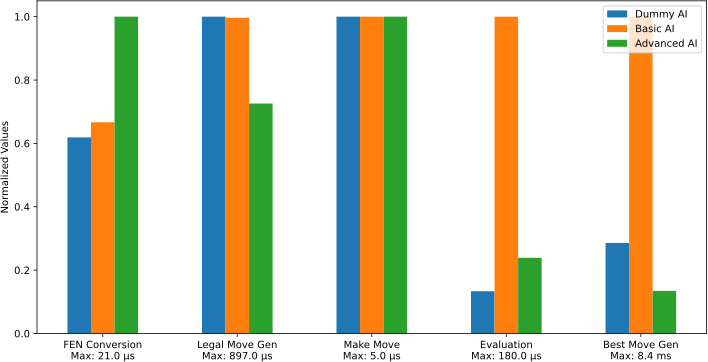
\includegraphics[width=.9\linewidth, page=1]{reference/pics/plot.pdf}
	\caption{Benchmarks of the different categories across the AI versions.}
	\label{fig:pillar-plot}
\end{figure}

The results are divided into five categories, with the first three determined by the chess backend and the latter two by the AI. It's important to note the significance of the legal move generation in the backend benchmarks. As the main bottleneck of the backend, any performance improvement in this area has a substantial impact on the overall performance of the AI. The reduction in time can be attributed to the refactoring process, which involved using lists of integers and minimizing boilerplate\footnote{
The Fen conversion is only used for debugging
purposes, the fact that it increased is not noticeable
in an optimized AI that doesn't debug anything.} code.

However, the most critical category is the final one, \textit{Best Move Generation}. As the name implies, this measures the speed at which the AI calculates the best move, in this case at a depth of one. Despite a slower evaluation compared to the previous version, the optimized AI demonstrates the best overall time. This underscores the fact that the final performance and strength of an AI are determined by multiple factors. In this instance, the number of nodes searched was significantly reduced by the implemented AI features, leading to an overall performance improvement.

This brings us to \autoref{fig:depth-plot}, which illustrates the relationship between time and the number of nodes searched in relation to the depths. As shown in the lower plot, the number of nodes searched is significantly lower for the optimized AI compared to the advanced AI\footnote{
The apparent lower number of nodes searched by the dummy and basic AI can be attributed to a bug in the early implementations of the AI related to move ordering. This issue was resolved in the third milestone. Therefore, the benchmarks for the dummy and basic AI in relation to depth should be interpreted with caution.
}. It's important to note that the apparent lower number of nodes searched by the dummy and basic AI is due to a bug in the early implementations of the AI related to move ordering, which was fixed in the third milestone. Therefore, the benchmarks for the dummy and basic AI in relation to depth should be interpreted with caution.

The plot also shows that the overall time is shorter for the optimized AI, regardless of depth. However, this is not always the case. For instance, if we had made poor decisions regarding the balance of exploration and exploitation in the MCTS, the performance could have actually been slower at higher depths. This highlights the importance of regular or atomic benchmarks, where a single element is changed to observe the system's response. Research also played a crucial role in fine-tuning the system.

\begin{figure}[hbtp]
	\centering
	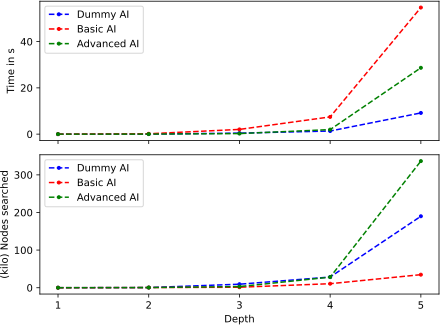
\includegraphics[width=.8\linewidth, page=1]{reference/pics/plot-depths.pdf}
	\captionsetup{justification=centering}
	\caption{Benchmarks of different AI versions in respect to search depth.\\Note that the number of nodes searched is in thousands (kilo).}
	\label{fig:depth-plot}
\end{figure}

\pagebreak


  \section{Issues faced}

  \section{Lessons learned}

  The process of writing a chess AI is not an easy one.
There are many things that can and will go wrong.
That's why this was a great way to learn,
because the first step to mastery is failure.
The following list is a collection of lessons we learned during
this project, they are in no particular order.

\begin{itemize}
  \item{
Benchmarks are extremely useful,
not only to see improvements over different versions of your code,
but also to compare incremental changes to the code.
We realized this when we tried to refactor the evaluation function to use numpy.
When we had many small np.ndarray it was actually slower then the pure python list implementation.
This is because we always have overhead when calling numpy,
so reducing the amount of times we call numpy draws out the full potential of numpy,
i.e. use as big as arrays as possible.
}
  \item{
We also observed that background tasks can significantly influence the result of benchmarks.
One should try to run them in the same-ish environment as possible
(or use a server for that if possible).
}
\end{itemize}

	
	\section{Summary}
	
	In this project we implemented our own chess AI and chess backend
in python. We had four milestones in total and the AI
got better with each. The final AI is able to play at a depth of 4 (plys)
in the mid-game. Some of the AI features we implemented are PeSTO,
MCTS, move ordering, Nullsearch and PVS/negamax.
We failed often, but learned from all of our mistakes.
Our team coordination was rough at first, but over time
it got better and better. In the final milestone
we were able to implement most features without any major
issues. Overall the learning experience was very positive
and build a really solid foundation for future projects.

	
	\addcontentsline{toc}{section}{Literatur}
	\renewcommand{\refname}{Literatur}
	\begin{thebibliography}{xxxx}
		\input{subfiles/sources.tex}
	\end{thebibliography}
	
\end{document}
